\chapter{定量脑电谱分析:基于EM算法的神经节律成分提取}

\section{引言}
神经震荡产生的兴奋和抑制塑造了大脑正常运行的传感、运动和认知过程。用新技术手段量化脑电磁记录的频谱曲线已成为研究神经震荡的主要方法之一。 一些存在的关于谱分解的文献报道了利用不具有合理统计学意义的准则来提取节律成分的手段。在本章中,我们利用Whittle似然准则和期望最大化算法分离和拟合谱曲线中的多个节律成分,我们分析发现“期望”步相当于维纳滤波(Wiener filtering)分离开多个节律成分,“最大化”步是最小化平滑惩罚和基于单调性形状约束的负Whittle似然函数,形状约束能够拟合多种不同形状的节律成分。谱曲线分解以后允许刻画各个节律的震荡幅度、共振频率、带宽、偏斜度、陡峭度和斜率。 这种方法称为$\xi\pi$模型,前后两个字母分别代表神经震荡
的背景活动和多种节律峰。 我们应用这种方法到大样本的颅内脑电数据集,从被试正常脑区的有限空间采样记录推断到未被记录到的脑区,最后得到了全脑高空间分辨率频谱参数成像。这种谱参数成像可能会为神经震荡和定量电生理研究提供了常模地形图,使我们对大脑动力学有了更进一步认识。

\section{研究背景}
神经震荡形成了细胞膜电位,再由神经元群的突触后电位同步活动累积成电流,最后被记录成为头表脑电(scalp EEG)、颅内脑电(iEEG)、皮层脑电(ECoG)和脑磁(MEG)信号\citing{buzsaki2012origin}。认知过程如注意、记忆、意识和脑功能失调的出现如精神紊乱、病态心理、精神分裂,以及皮层网络的本质都可以通过对神经震荡的研究进一步解释\citing{buzsaki2004neuronal,
uhlhaas2006neural,uhlhaas2010abnormal,ward2003synchronous}。脑电磁记录的谱分析提供了大尺度神经震荡的“指纹”特征\citing{siegel2012spectral}。

当定量脑电\citing{john1977neurometrics,da1974model,zetterberg1969estimation}的概念在19世纪70年代被提出的同时,
建立能够进行频谱分解和刻画大脑节律特征的模型也成为热门研究问题。Zetterberg等利用了滤波器的概念识别频谱中的三种成分类型并用最大似然估计法估计成分的参数\citing{isaksson1981computer,wennberg1971application,
zetterberg1975analogue}。随着定量脑电中计算机辅助分析诊断\citing{john1988neurometrics}的出现,Pascual等在\cite{pascual1988parametric}提出了基于似然比检验的方法,命名为$\xi\alpha$模型,用以提取背景震荡活动$\xi$和$\alpha$节律的参数,并应用该方法到多通道谱分析。 $\xi\alpha$模型用Student-t型分布曲线\citing{walpole2011probability,
fisher1925applications,senn1994first}拟合每一个成分,频谱中只有$\alpha$峰被拟合到,该模型没有考虑其他频带的谱峰。 最近,FOOOF通过用启发式反馈拟合的方式最小化残差平方和能够拟合出1/f震荡过程的参数和不同频带多个谱峰的高斯核参数\citing{haller2018parameterizing}。

然而,我们还可从如下几点思考存在方法的不足:
1)我们还不清楚背景谱震荡是否适合描述为1/f过程\citing{abry1995wavelets}; 2)由于谱曲线上多个频带区间上谱峰形状不一,以前采用的参数化拟合例如t型曲线或者高斯核能够有效地拟合到所有的谱成分吗? 3)比着FOOOF中用的最小二乘,是否有其他更加理论合理的准则賴评估谱曲线拟合的优劣?
4)在某个认知过程中存在多少个节律(谱峰),或者说给定一个谱曲线我们要用多少谱峰来拟合?

为了回答单个谱峰形态各异的拟合问题,平滑的单模态回归由于非参数的性质和在形状上灵活的约束似乎是一个有效的方法\citing{eilers2005unimodal,pya2015shape}。 考虑到谱成分的形态各异的特性,背景震荡仅仅是一个单调下降的函数,各个谱峰可以看作先单调上升到谱峰位置再单调下降的函数。 为了找到谱估计的合理准则,Whittle似然利用单个频率下的傅里叶系数基于中心极限定理是圆周复正态分布的假设是谱成分的统计学一致的估计量\citing{whittle1953estimatio,whittle1951hypothesis}。 谱曲线拟合的关键之一是谱峰的个数,一般可以从: i)数据驱动,谱峰的个数就是出现在谱曲线中的波峰的个数, 被一个稍微的波谷隔开的相近两个波峰即视为两个谱峰,在这种情况下,最佳的拟合通过最大似然估计或者最小化残差平方和获得;ii)模型驱动,谱峰的个数不依赖于视觉上的多少,不同频带的谱峰可能是谐波,谱峰之间可能累加或者相互抵消,被稍微的波谷隔开的相近波峰可视为一个连续大谱峰,这需要从以前的神经震荡研究中获取更多的先验知识,在这种情况下最小化拟合的残差平方和可能出现过拟合或者拟合不足,这可能通过结合神经生理学先验设计出用组稀疏(group lasso\citing{yuan2006model})的期望最大化算法。
\begin{figure}
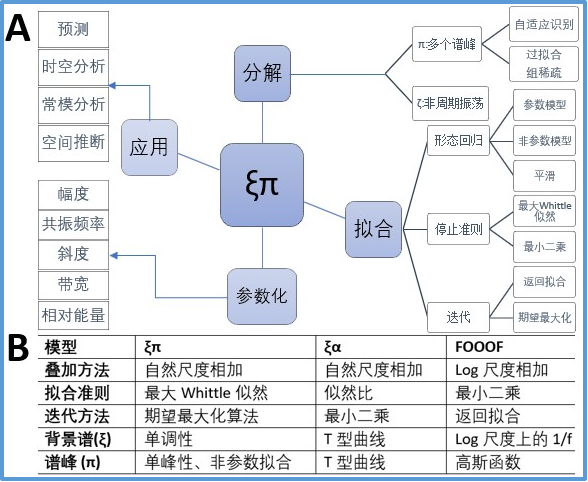
\includegraphics[width=15cm]{pic/xipi/model.png}
\caption{量化神经震荡谱曲线的$\xi\pi$模型。 A:$\xi\pi$模型综合视角,B:$\xi\pi$模型与$\xi\alpha$模型、FOOOF模型的方法比较。}
\label{model}
\end{figure}

除了神经震荡谱曲线的拟合和分解,解码(量化)神经震荡谱曲线应该如\ref{model}中所示按照整体系统的观点进行。拟合和分解把神经谱曲线分成几个谱成分的和,这很接近于逆问题,利用主要最小化(majorization-minimization)算法\citing{Demidenko2004,mclachlan2007algorithm,zhou2019mm,sun2016majorization}的特例期望最大化算法求解具有优势。 从谱成分中提取的参数是对神经振荡有解释意义的变量如震荡幅度、共振频率、带宽、偏斜度、陡峭度、斜率和相对于总能量的谱能量。 这使得$\xi\pi$模型应用于 1)用大型正常人群数据建立头表和源空间的震荡谱特征常模;2)作为预测认知过程和分类诊断情感紊乱的标记物;3)用iEEG或ECoG数据进行某些被试记录脑区到另一些被试未被记录到的脑区的推断\citing{owen2017towards},得到全脑高分辨率谱参数成像,
这可能为脑电磁源成像提供常模。

在本章中,我们发现谱曲线拟合的“期望”步骤相当于Wiener滤波器来分析不同的谱成分,“最大化”步骤是通过最小化单调性形态和平滑约束的Whittle似然函数来拟合每个谱成分。 利用公开的iEEG数据\citing{frauscher2018atlas,owen2017towards},我们希望得到一种全脑空
间的高分辨率谱参数成像。

\section{研究数据与方法}
\subsection{数据}
我们访问到加拿大蒙特利尔神经病学研究所公开的颅内正常脑电数据集\citing{frauscher2018atlas}。该数据库收集了来自加拿大和法国
三家医院106位癫痫病人(女:54位,年龄均值33.1$\pm$10.8)被试在接受颅内手术治疗时植入在正常脑区的电极在病人非癫痫发作的清醒安静闭眼状态下记录的脑电数据。每个被试的电极位置不同,106位被试的电极总数达到1785,1785个电极位置被定位到共同的立体定向空间中,便于综合分析。1785通道脑电数据经电生理专家视觉筛选,得到60s没有噪声的数据。颅内脑电数据采集采用每个电极上的双极参考。其中89个被试采用立体空间穿刺电极(共1520个)、17位被试采用覆盖皮层表面的条状或栅格片状电极(共265个)。 左侧大脑半球电极覆盖1066
个,右侧719个,大脑灰质和皮层表面的电极覆盖率分别为每$cm^3$2.7和0.9个。全脑被自动划分为38个脑区,每个脑区上的电极数目范围
为6-178个。 106被试结构数据与电极位置的配准到共同的ICBM152\citing{mazziotta2001probabilistic,fonov2011unbiased}立体空间的所有电极位置的位置和分区如图\ref{electrodes}所示。
\begin{figure}
\includegraphics[width=15cm]{pic/xipi/electrodes.png}
\caption{颅内正常脑电数据集的电极分布与分区。黄色点表示电极位置。前两列从左到右从上到下分别表示左右半球的外侧和内侧视图,第三列的上下两图分别表示自头顶向下和自下向头顶的试图,最后一列表示左右半球的分区。}
\label{electrodes}
\end{figure}

\subsection{谱曲线分解}
我们首先对脑电磁数据分段,再对每一段进行FFT变换得到傅里叶系数。 如果$y_\omega$是数据段$s(s=1,...,N_s)$在频率$\omega(\omega=1,...,N_\omega)$处的傅里叶系数,$\mathbf{z}\in{\mathbb{R}^{N_k\times{1}}}$是全为1的向量,用以进行$N_k$个$\mathbf{b}_\omega\in{\mathbb{C}^{N_k\times{1}}}$包含了在数据段s和频率$\omega$时对应于$N_k$个成分的傅里叶系数,$\Sigma_\omega=diag(\sigma_\omega)$,$\sigma_\omega=[\sigma_\omega^1,...,\sigma_\omega^{N_k}]^T$,$\epsilon_\omega\sim{N^\mathbb{C}(0,\sigma_\epsilon)}$是所有频率上具有常数方差的傅里叶系数分解残差,那么傅里叶系数分解模型是
\begin{equation}\label{eq1}
y_\omega=\mathbf{z}^T\mathbf{b}_\omega+\epsilon_\omega
\end{equation}
估计的谱是所有数据段上傅里叶系数的样本方差
\begin{equation}\label{eq2}
s_\omega=\frac{1}{N_s}\sum_{s=1}^{N_s}y_{\omega,s}^*y_{\omega,s}
\end{equation}
指定实际中计算得到的谱为$s_\omega$,理论上待拟合的谱为$\sigma_\omega$,Whittle似然\citing{pawitan1994penalized,
whittle1953estimatio,whittle1951hypothesis}定义为
\begin{equation}\label{eq3}
\ell_\omega=\sum_{\omega=1}^{N_\omega}\lbrace\log{\sigma_\omega}+\frac{s_\omega}{\sigma_\omega}\rbrace
\end{equation}

给定观测模型\eqref{eq1},脑电谱曲线分解转换为对傅里叶系数$\mathbf{b}_\omega$的估计。 利用方差成分模型和期望最大化
算法\citing{mclachlan2007algorithm},未知参数的向量为$\mathbf{\theta}_\omega^{i}=(\mathbf{\sigma}_\omega^{i};\sigma_\omega^{i})$,则完全负$\log$似然表达式为
\begin{equation}\label{eq4}
\ell_c=\sum_{\omega=1}^{N_\omega}\sum_{s=1}^{N_s}\lbrace\log{\sigma}_\epsilon^{(i)}+\mathbf{\sigma}_\epsilon^{(i)-1}\mathbf{\epsilon}_\omega^{(i)*}\mathbf{\epsilon}_\omega^{(i)}+\log\lvert\Sigma_\omega^{(i)}\rvert+\mathbf{b}_{\omega,s}^{(i)*}\Sigma_\omega^{(i)-1}\mathbf{b}_{\omega,s}^{(i)}\rbrace
\end{equation}

\subsubsection{期望步骤}
\eqref{eq1}中$y_\omega$的方差是$c_\omega^{(i)}=\Sigma_{k=1}^{N_k}\sigma_\omega^{k(i)}+\sigma_\epsilon^{(i)}$。 根据最小模最小二乘解和矩阵逆引理\citing{tarantola_inverse_2005},我们得到
\begin{equation}\label{eq5}
\mathbf{E}_{\mathbf{\theta}_\omega^{(i)}}(b_\omega^{k(i)}\mid{y}_\omega)=\sigma_\omega^{k(i)}c_\omega^{(i)-1}y_\omega
\end{equation}

显然,这里频谱中的傅里叶系数分解是一个Wiener滤波\citing{kalman1960new,Wiener1949}问题。在期望步骤,我们也可以推出
\begin{equation}\label{eq6}
d_\omega^{k(i)}=\mathbf{E}_{\mathbf{\theta}_\omega^{(i)}}(b_\omega^{k(i)}b_\omega^{k(i)*}\mid{s}_\omega)=\sigma_\omega^{k(i)}+(s_\omega-c_\omega^{(i)})c_\omega^{(i)-2}\sigma_\omega^{k(i)2}
\end{equation}
\begin{equation}\label{eq7}
e_\omega^{(i)}=\mathbf{E}_{\mathbf{\theta}_\omega^{(i)}}(\epsilon_\omega^{(i)}\epsilon_\omega^{k(i)*}\mid{s}_\omega)=\sigma_\epsilon^{(i)}+(s_\omega-c_\omega^{(i)})c_\omega^{(i)-2}\sigma_\omega^{(i)2}
\end{equation}

\subsubsection{最大化M步骤}
条件完全负$\log$似然函数是
\begin{equation}\label{eq8}
Q(\mathbf{\theta},\mathbf{\theta}^{i})=\sum_{\omega=1}^{N_\omega}\lbrace\log{\sigma_\epsilon}+\sigma_\epsilon^{-1}e_\omega^{(i)}+\sum_{k=1}^{N_k}(\log{\sigma}_\omega^k+\sigma_\omega^{k-1}d_\omega^{k(i)})\rbrace
\end{equation}
这里$\sigma_\omega^{k(i+1)}$是对$d_\omega^{k(i)}$的近似估计量,通过平滑形态约束的Whittle似然函数来拟合。

假设\eqref{eq1}中傅里叶系数分解残差的方差对所有频率上是常量,在最大化步骤可以计算为
\begin{equation}\label{eq9}
\sigma_\epsilon^{(i+1)}=\frac{1}{N_\omega}\sum_{\omega=1}^{N_\omega}e_\omega^{(i)}
\end{equation}

\subsubsection{不完全似然函数}
\begin{equation}\label{eq10}
\ell_{ic}=\sum_{\omega=1}^{N_\omega}\sum_{s=1}^{N_s}\lbrace\log{\sigma_\epsilon^{(i+1)}}+\frac{\epsilon_\omega^{(i)*}\epsilon_\omega^{(i)}}{\sigma_\omega^{(i+1)}}\rbrace
\end{equation}
直到不完全似然函数收敛,期望最大化算法完成迭代。

\subsection{谱成分拟合}
谱成分拟合指的是谱曲线分解最大化步骤对$d_\omega^{k(i)}$的拟合。如果将所有频率下对应的标量存为向量,我们得到$\mathbf{b}^{k(i)}=[d_1^{k(i)},...,d_\omega^{k(i)},...,d_{N_\omega}^{k(i)}]^T$和$\mathbf{\sigma}^{k(i+1)}=[\sigma_1^{k(i+1)},...,\sigma_\omega^{k(i+1)},...,\sigma_{N_\omega}^{k(i+1)}]^T$。\eqref{eq3}中的Whittle似然可以进一步
表示为:
\begin{equation}\label{eq11}
\ell_\omega^{(i+1)}=\mathbf{1}^T(\log{\mathbf{\sigma}}^{k(i+1)}+\mathbf{d}^{k(i)}\bigodot{\mathbf{\sigma}^{k(i+1)-1}})
\end{equation}

使用平滑形态约束\citing{eilers2005unimodal,wahba1980automatic}对$\mathbf{\sigma}^k$的估计,目标函数是
\begin{equation}\label{eq12}
\hat{\mathbf{\sigma}}^{k(i+1)}=arg\min_{\mathbf{\sigma}^{k(i+1)}}\ell_\omega^{(i+1)}+\lambda\lVert\mathbf{D}_3\mathbf{\sigma}^{k(i+1)}\rVert_2^2\quad
s.t.\;\mathbf{\sigma}^{k(i+1)}>\mathbf{0},\mathbf{D}_1\mathbf{\sigma}^{k(i+1)}<\mathbf{0}
\end{equation}

这里$\lambda$是调整平滑程度的参数,$\mathbf{D}_3$是三阶差分矩阵平滑算子,$\mathbf{D}_1$是(修正的)一阶差分矩阵梯度算子。如果$d^{k(i)}$是单调递减曲线,$\mathbf{D}_1$就是一阶差分矩阵梯度算子,对于谱峰成分,
$\mathbf{D}_1$在谱峰最大值左侧的元素反转正负号,即谱峰最大值左右在梯度算子中分别具有负梯度和正梯度。 在对非周期震荡谱成分$\xi$和周期节律震荡谱成分$\pi$的拟合中,我们采用的调整平滑度的参数分别为0.1和$10^{-5}$,这些参数是经过一定范围搜索后得到,实际中是否使用平滑度参数的精确值对谱拟合的效果影响不大,主要作用在保证单调性形态约束的前提下微调平滑性。

\subsection{谱拟合误差}
对于每一个电极上的谱曲线,记实际的待拟合的谱曲线为Spt、拟合的谱曲线为Fit,则拟合误差计算为
\begin{equation}\label{eq13}
RE = \frac{\lVert{Spt-Fit}\rVert_2}{\lVert{Spt}\rVert_2}
\end{equation}

\subsection{参数量化}
尽管我们在期望最大化算法的最大化步骤中采用了非参数拟合的方法拟合出单个谱成分。 为了量化谱成分,我们需要逐一提取单个谱成分的参数。考虑到每一个谱成分的曲线只代表了某个特定频率下特定电极位置的震荡事件,我们面对样本量少且群体标准偏差未知的情形,但谱曲线是接近高斯分布的铃形曲线,可以采用Student t型的概率密度曲线,用式子表示为
\begin{equation}\label{eq14}
f(\omega)=a/\lbrace1+[(\omega-\mu)^2/\tau]^2\rbrace^{\exp^\upsilon}
\end{equation}
这里$f$是谱成分在频率$\omega$时的功率谱大小,$a$、$\mu$、$\tau$、$\upsilon$分别是该谱成分的震荡幅度、参数包括最大谱震荡幅度
、共振中心频率,幅半频带宽度和斜率。 这里我们采用了类似与$\xi\alpha$模型\citing{pascual1988parametric}的参数提取方法。

\subsection{基于高斯过程回归绘制皮层震荡谱图}\label{ch:kriging}
给定颅内某些位置上的脑电谱数据,提取到的参数是一些特定空间位置上在特定频率点形成的震荡。为了获取任意空间位置任意频率下的谱值,借助地质空间统计学的空间插值方法,我们采用高斯过程回归(又称为Kriging方法)根据已知参数估计未知参数。

\subsubsection{大脑皮层空间几何学处理}
根据\cite{frauscher2018atlas}中的描述,作者首先使用\href{www.bic.mni.mcgill.ca/ServicesSoftware/Services SoftwareMincToolKit}{Minctools}和IBIS架构\citing{drouin2017ibis}将颅内电极的解剖位置配准到立体空间中,接着将每个病人的颅内手术中显示有电极位置的CT或者MRI图像与病人手术前的MRI图像线性配准。手术前的MRI图像非线性地配准到ICBM152非线性对称脑模型\citing{mazziotta2001probabilistic,fonov2011unbiased}这些配准使得来自106病人正常脑区的电极累积为总数为1785个电极集,这些
电极几乎覆盖全脑,配置使得所有电极变换到共同的三维立体空间,便于对大量正常脑电活动进行组分析和可视化。

我们访问得到iEEG数据集去只提供了1772个电极的脑电数据(去除了13个,原因未知),提供的配准到ICBM152头模型具有238436体素点,远超过电极数目1772,这样多个相近的体素点可能位于同一个电极周围。在此基础上,我们为了提高从有限电极观测到全脑空间的估计准确性,按照MATLAB中reducepatch方法将左右脑半球的网格三角形面的个数都减少到6000,空间降采样后全脑的网格顶点为$N_v=6004$个。 根据1772电极位置和全脑6004个网格顶点位置的坐标,我们找到离每个电极位置空间欧式距离最近的大脑中网格顶点。按照全脑皮层中网格顶点形成三角形面相互连接的关系,我们首先建立权重为非0即1的对称连接矩阵6004x6004,根据该连接矩阵得到了无向连接图,基于此图和Dijkstra算法\citing{dijkstra1959note}计算得到全脑网格两两顶点之间的最短路径长度矩阵,记为$\mathbf{G}\in{\mathbb{Z}^{N_v\times{N_v}}}$。

\subsubsection{高斯过程回归超参数选择}
记所有电极上的谱成分个数为$K=\sum_{e=1}^{1772}k_e$,所有谱成分所在大脑网格顶点之间的最短路径长度矩阵为$\mathbf{G}_v\in{\mathbb{Z}^{K\times{K}}}$,所有谱成分共振频率间隔$\mathbf{G}_\mu\in{\mathbb{R}^{K\times{K}}}$,所有谱成分的震荡幅度
为$\mathbf{a}\in{\mathbb{R}^{K\times1}}$,谱成分关于路径长度和共振频率间隔的偏差分别为$\lambda_d$、$\lambda_\mu$。在谱成分分离以后,我们可知每个电极的谱成分个数k和每个谱成分的共振频率$\mu$,按照逐一电极的顺序对每一个谱成分标定距离最近
的大脑网格顶点$\mathbf{v}\in{\mathbb{Z}^{K}\times1}$,并计算出所有谱成分共振频率间隔矩阵。超参数的选择表示为

\begin{equation}\label{eq15}
\begin{split}
\mathbf{G}_v& = \mathbf{G}(v,v)^{\circ2}\\
\mathbf{W}& =\exp^{(-\frac{\mathbf{G}_v}{\lambda_d}-\frac{\mathbf{G}_\mu^{\circ2}}{\lambda_\mu})}-\mathbf{I}_K\\
\tilde{\mathbf{a}}& =\mathbf{W}\oslash{(\sum_{k=1}^K\mathbf{W}(:,k))\mathbf{1}^T}\mathbf{a}\\
(\tilde{\lambda}_d,\tilde{\lambda}_\mu)& =arg\min_{\lambda_d,\lambda_\mu}\sqrt{{\frac{\sum_{k=1}^{K}(\tilde{a}_k-a_k)}{K}}^2}
\end{split}
\end{equation}

\subsubsection{全脑空间谱估计与地形图绘制}
设预插值估计频率点为$\omega$,该频率点下全脑空间所有网格顶点上谱值为$\mathbf{p}_\omega$,则
\begin{equation}\label{eq16}
\begin{split}
\mathbf{G}^\prime_v& = \mathbf{G}(:,v)^{\circ2}\\
\mathbf{G}^\prime_\mu& = \mathbf{1}_{N_v}(\mathbf{\mu}^T-\omega)^{\circ2}\\
\mathbf{W}& =\exp^{(-\frac{\mathbf{G}^\prime_v}{\tilde{\lambda}_d}-\frac{\mathbf{G}^\prime_\mu}{\tilde{\lambda}_\mu})}\\
\mathbf{p_\omega}& =\mathbf{W}\oslash{(\sum_{k=1}^K\mathbf{W}(:,k))\mathbf{1}^T}\mathbf{a}
\end{split}
\end{equation}
利用全脑的网格顶点和三角形面信息,我们可以将任意频率下的谱值$\mathbf{p_\omega}$绘制到三维空间地形图上。

\section{研究结果与讨论}
\subsection{初始化拟合}
适当的初始化参数选择是使用期望最大化算法,减少迭代次数,保证收敛到全局最优点的关键。因为期望最大化算法是一种聚类数目已知的成分混合模型,但在谱曲线拟合中每个电极位置的谱曲线中的谱峰的个数以及频率位置未知,我们无法给定先验地确定谱成分的个数。因此,进行初始化的必要任务是确定谱曲线中的谱成分的个数。我们发现MATLAB的信号处理工具箱中对测量信号进行特征提取的描述统计学函数之一findpeaks能够较好地完成谱峰提取的任务。findpeaks具有最大峰值个数、最小峰值高度、最小峰值相对重要性、最小峰值高度差、最小和最大峰值宽度等参数。其中最小峰值相对重要性参数定义了谱峰下面积相对于周围其他谱峰的重要性,在本章研究中一般设为0.02。 峰值高度和宽度可作为辅助参数,因为谱曲线高度受到最大谱值的影响,我们对谱曲线按照最大谱值归一化,设最小峰值高度为0.06、最小峰值宽度为0.2。图\ref{detect}是使用该函数和上述参数在一例真实脑电谱曲线中提取的谱峰和谱谷的位置。从图中可以看出,findpeaks能够较好地抓取到谱峰的位置。根据谱峰的位置、高度以及findpeaks函数返回的每一个谱峰的宽度等参数,我们可以通过t型曲线来初步拟合出每一个谱成分的曲线。
\begin{figure}
	\includegraphics[width=15cm]{pic/xipi/detect.png}
	\caption{初始化获取谱峰、谱谷的位置。Spt:从一例实际脑电数据分析得到的谱曲线,Pks:谱峰位置,Vlys:谱谷位置。}
	\label{detect}
\end{figure}

\subsection{$\xi\pi$与FOOOF拟合效果比较}
在能够进行谱曲线拟合和成分节律提取的方法中,Zetterberg等的方法\citing{isaksson1981computer,
wennberg1971application,zetterberg1975analogue}是基于滤波器设计,Pascual的方法\citing{pascual1988parametric}只能拟合$\alpha$节律谱峰和背景非谱峰成分,A. K. I. Chiang的方法\citing{chiang2008automated}只是对$\alpha$频带的谱峰分解为多个子谱峰,只有Haller等的方法FOOOF\citing{haller2018parameterizing}可以拟合多种谱峰和背景非谱峰
成分。

FOOOF模型是首先对实际谱数据作$log_{10}$变换,再对背景震荡和谱节律成分按照自然尺度分别拟合。与之不同,$\xi\pi$模型直接在原始
谱曲线的自然尺度上进行分解和拟合,为了与FOOOF模型的工具包结果形成对比,我们也将$\xi\pi$在自然尺度上拟合得到的结果作$\log_{10}$变换再画在$\log_{10}$尺度上。图\ref{comp}D是我们使用FOOOF模型的\href{https://github.com/fooof-tools/fooof/tree/master/fooof}{基于Python语言的工具包}对一例实际脑电谱数据拟合输出的原始图。使用$\xi\pi$模型得到的结果与FOOOF模型的效果比较
分别表示在图\ref{comp}ABC中,依次是全模型对谱曲线的整体拟合效果、对背景非周期震荡曲线的拟合效果和对周期节律震荡谱峰成分的拟
合效果。从图\ref{comp}A中可以看出,$\xi\pi$模型得到比FOOOF模型较好的拟合,拟合出的谱曲线基本上和实际的相重合,相比之下,
FOOOF模型拟合出的曲线严重偏离了实际谱曲线。在图\ref{comp}B中,$\xi\pi$模型拟合出的非周期背景震荡谱曲线较好地吻合了实际谱曲线的背景震荡非谱峰位置,然而FOOOF模型甚至在低频处拟合出了比实际高很多、在高频处比实际低很多的曲线。$\xi\pi$模型与FOOOF对周期
节律震荡谱成分的效果对比也容易看出$\xi\pi$模型在全频带上都有信号,特别是谱峰幅度小于1时也随着频率而变化,谱峰的位置较好地出
现在如图\ref{detect}中自然尺度上谱峰的下方位置,然而因为FOOOF模型是先对谱曲线做$log_{10}$变换再进行拟合,所以FOOOF模型拟
合出的$log_{10}$尺度上谱峰成分在谱峰的位置周围都为0。 总体上$\xi\pi$的拟合出的谱曲线较好地保持了实际谱曲线的细节轨迹变化,只是非周期的背景震荡成分是单调下降的曲线,对于谱峰成分的拟合,在全频带上都拟合出了随着频率变化体现几个共振频率下的谱峰的结合趋势,这是$\xi\pi$模型中使用的非参数拟合和单调性约束的结果,然而FOOOF模型拟合曲线表现出较强的平滑性,无论在背景震荡还是节律谱成分震荡曲线拟合上都表现出了某种形状,这种形状是由高斯核的参数拟合造成的。显然,$\xi\pi$模型的非参数拟合得到了比FOOOF模型在本例中非对称形状且左右瓣凹凸性不一致的谱峰更好的拟合效果,而FOOOF对每个谱峰拟合出的左右瓣都是两两对称且向外凸。
\begin{figure}
	\includegraphics[width=15cm]{pic/xipi/comp.png}
	\caption{$\xi\pi$模型与FOF模型的拟和效果比较。 Spt: 原始谱曲线,$\xi\pi$:本文中提出的模型,FOF:FOOOF model\citing{haller2018parameterizing}。A. 模型总体拟合效果比较,B.背景震荡拟合效果比较,C.谱峰拟合效果比较,D.使用FOF Python工具包拟合结果原图,纵坐标的Power实际上是对原始谱曲线求$log_{10}$之后的值}
	\label{comp}
\end{figure}

\subsection{$\xi\pi$模型的拟合过程与分解效果}
为了更进一步了解$\xi\pi$模型的拟合过程和成分分解效果,我们将与上述两节中相同的实际脑电谱数据的不同迭代拟合结果和负似然函数变
化表示在图\ref{allinone}AB中。 从B中我们可知负似然函数随着迭代次数下降,表明了模型中使用期望最大化算法进行迭代拟合和分解的有效性。在实际模型计算中,我们发现负似然函数有时难以收敛,但是10次左右迭代后的拟合出谱曲线已经与实际的谱曲线较好的吻合。负似然函数还未收敛的原因是模型为了拟合出某些尚未拟合好的细节,然而,这些未拟合好的细节正式由于模型中引入的基于单调性的形态约束造成的,因此过度地追求目标函数的收敛已经无太大意义。拟合效果随着迭代变化趋势如图\ref{allinone}A中所示,容易看出,根据findpeaks
进行初始化的结果已经接近实际的谱曲线,$\xi\pi$模型中的期望最大化算法的作用是对初始化的结果进行迭代调整。根据经验,如果负似然函数在迭代次数超过50次后不收敛,我们会终止迭代,取所有迭代中拟合出的谱曲线与实际谱曲线相对误差(RE)最小值。图\ref{allinone}B中表示了对该实际脑电谱曲线的总体拟合和分解效果,蓝色的原始谱曲线被深蓝色的拟合出的谱曲线几乎完全覆盖,深蓝色拟合出的谱曲线是表示非周期背景震荡的$\xi$与周期节律震荡$\pi$($\theta$、$\alpha_1$、$\alpha_2$、$\beta_1$、$\beta_2$)的成分线性叠加后的
结果。$\xi\pi$模型的主要目标之一就是将实际的谱曲线分离为非周期震荡和若干代表节律震荡的谱峰成分。
\begin{figure}
	\includegraphics[width=15cm]{pic/xipi/allinone.png}
	\caption{$\xi\pi$模型的迭代和总体分离效果。A.迭代拟合,Init:根据findpeaks进行初始化的结果,i=1,5,10表示第1、5、
	10次	迭代。 B.负的log似然函数随迭代次数的变化。 C.最终总体拟合与分离效果,$\alpha_1$、$\alpha_2$、$\beta_1$、$\beta_2$表示$\alpha$、$\beta$频带的第1、2个谱峰成分。}
	\label{allinone}
\end{figure}

\subsection{颅内脑电谱参数提取}
我们对1772个电极上的脑电信号进行谱分析,根据student t型曲线提取出了震荡谱成分震荡最大幅度$a$、谱成分共振中心频率$\mu$、谱成
分幅半频带宽度$\tau$和斜率$\upsilon$。虽然每个电极上谱曲线的谱成分个数不同,但我们根据\cite{frauscher2018atlas}中报道的结
果作为先验知识,设置谱曲线中的最大成分数为15。图\ref{para}A中左右两图分别表示了$\xi\pi$模型对1772个电极谱曲线拟合相对误差随
谱曲线成分个数的变化直方图和1772个电极谱曲线拟合误差关于电极数目的归一化后的直方图。从图\ref{para}A左图中可以看出极少比例的电极上谱曲线仅仅具有非周期震荡不具有节律震荡,大部分电极上具有2-6个谱成分,还有一部分具有7个及以上谱成分。图\ref{para}A右图
中直方图表明了所有电极上拟合误差在0.1(10\%)左右,对应左图中较亮颜色(红黄白色)处的RE,说明总体上具有较好的拟合效果。

图\ref{para}中BC两行自左向右分别表示节律周期震荡谱峰成分$\pi$和非周期震荡背景谱成分$\xi$中最大震荡幅度$a$随震荡中心频率$\mu$的直方图、最大震荡幅度$a$随震荡频率幅半带宽$\tau$的直方图、斜率$\upsilon$随震荡频率幅半带宽$\tau$的直方图。从BC两行的第一列上下两图可以看出节律震荡在8、12、22Hz左右形成较强的谱峰,非周期背景震荡在最小频率分辨率电0.39Hz处具有最大震荡幅值,这与文献\cite{frauscher2018atlas}报道的谱峰频率位置相吻合,以及与非周期背景震荡在最低频率点具有最大震荡幅度的认识相一致;从BC两行的第二列的上下两图中观察发现非周期背景谱成分和节律谱峰成分的最大震荡幅值都随着带宽增加而下降,这与物理学中的震荡谱能量呈现1/f类型的幂律分布相吻合;从BC两行的第三列两图中可以看出斜率都随着震荡带宽增加而上升,但节律周期震荡斜率在大多数情况下大于非周期背景震荡的斜率,这一点与\cite{pascual1988parametric,amador1989structure,amador1990spatiotemporal}报道的周期震荡用斜率60远大于非周期震荡用的斜率1.5的结果类似;这也和周期节律震荡表示系统中不稳定的随机突发性震荡事件有关、背景非周期震荡表示系统中稳定的可能是噪声的活动有关,不稳定的随机突发性震荡事件的谱曲线类似于窄带脉冲具有远大于稳定的非周期噪声的宽带震荡的斜率。
\begin{figure}
\includegraphics[width=15cm]{pic/xipi/para.png}
\caption{1772个电极谱拟合与参数提取。A行:左图表示拟合误差随着电极上拟合出的谱成分个数变化的直方图,右图表示1772个电极上谱成分的拟合误差直方图;B行表示谱峰$\pi$成分拟合情况,左图表示参数$a$随参数$\mu$的直方图分布,中图表示参数$\mu$随参数$\tau$的直方图分布,有图表示参数$\upsilon$随参数$\tau$的直方图分布;C行表示背景震荡$\xi$的拟合情况。 所有直方图的颜色尺度相同。}
\label{para}
\end{figure}

\subsection{全脑空间谱地形图}
对全脑空间中部分位置采样的1772个电极的谱曲线拟合并提取成分参数之后,我们采用描述在\ref{ch:kriging}一节中基于高斯过程回归的
方法估计任意频率任意全脑空间网格顶点位置上的震荡谱值。 以2、5、10、26Hz为代表,我们分别估计得到对于$\delta$(1-3Hz)、$\theta$(4-7Hz)、$\alpha$(8-12Hz)、$\beta$(16-30Hz)的传统频带的节律的最大震荡谱值分布,并根据全脑空间的网格顶点和三角形面信息将分
布结果画在图\ref{map}中的大脑皮层的空间地形图上。注意到图\ref{map}中每一列对于一个频带,自上向下分别是顶测、左侧、右侧视图。 同时,不同频带的空间地形图的颜色尺度不同,从低频到高频,颜色尺度的最大最小值范围逐渐下降。我们发现$\delta$节律的震荡分布在前
额叶、左侧枕叶和双侧颞叶,$\theta$节律的震荡主要分布在右侧上额回、右侧辅助运动区、右侧前后中央回、左侧枕叶和左侧前额叶,
$\alpha$节律的震荡主要分布在左右双侧颞叶、左右双侧枕叶和左侧顶叶、$\beta$节律的震荡主要分布在左右双侧上额回、左右双侧前后
中央回和左侧辅助运动区,集中在前额叶和顶叶,呈现双侧对称分布。 总结起来,$\delta$、$\theta$、$\beta$节律的分布更为分散,而$\alpha$节律的分布主要集中在后中央回以下的顶枕叶,但枕叶全部并非只有$\alpha$节律,在部分枕叶区域也可能出现$\delta$和$\theta$节律。这些结果与报道在\cite{gastaut1949enregistrement,jasper1949electrocorticograms,sem1953depth,chatrian1960depth,sem1956electroencephalographic,perez1962electrographic,graf1984electrocorticography,frauscher2018atlas}中的结果相吻合。 基于$\xi\pi$模型和斯过程回归的方法,我们将对颅内正常脑区空间有限采样的脑电信号谱曲线分解提取出各个谱成分的
参数并进行频率和大脑空间位置上的插值,得到了与文献中以报道的结果相一致的结果,这种频率和大脑空间两个维度上的高分辨率神经震荡节律谱地形图为提供了正常脑电的谱地形图常模大脑源空间曲面,可能为脑电溯源方法研究提供基准,为源空间下的定量脑电、异常脑电分析提供了一种参考。

\begin{figure}
	\includegraphics[width=15cm]{pic/xipi/map.png}
	\caption{全脑空间谱地形图。从左到右分别是$\delta$(2Hz)、$\theta$(5Hz)、$\alpha$(10Hz)、$\beta$(26Hz)处的谱地形图,前三行自上向下分别是顶测、左侧、右侧视图,各个频带对于不同的颜色尺度。}
	\label{map}
\end{figure}

\section{讨论}
There are a few problems remained to solve: (1) Add the constraint σ > 0 when using Whittle likelihood at
ordinary scale. (2) To tune the smoothing parameter, how to calculate the degree of freedom of a
nonparametric fitting? divergence of MLE (Monto Carlo)? (3) Can Whittle likelihood be transformed into a least
square, via series expansion or by log transformation (check the expansional family)? (4) Organize the Bayesian
and spectrum papers in Mendeley. (5) Review Bayesian analysis, projection estimator, Wahba smoothing and
Whittle likelihood.
The developer version of the Xi rhythms toolbox is at https://github.com/ShiangHu/SCMOPT.git.
author/funder. 

\section{本章小结}
本章中,我们使用期望最大化算法和基于单调性的形态回归提出了能够有效分解谱曲线多个谱峰与非周期震荡谱并提取谱成分特征的模型,称为$\xi\pi$模型。 这种模型与前人提出的方法的主要不同在于使用了基于Whittle似然这种更加具有谱估计拟合统计学理论意义的准则,利用不完全数据的方差成分模型和期望最大化算法,对每一个成分的拟合首次采用了只从形态意义上约束单调性的非参数拟合。 我们应用这种$\xi\pi$模型取得了比当前引人注意的基于高斯核拟合的FOOOF模型更好的估计,证明了FOOOF模型在$\log_{10}$尺度上进行参数拟合的缺点。 应用$\xi\pi$模型到1772正常颅内脑电数据集上,我们得到了一种高频率和空间分辨率的全脑空间节律震荡谱地形图,为利用溯源方法基于源空间的谱分析进行定量脑电研究提供了基础。